This chapter will provide the reader with an overview of the relevant parts of Java HotSpot. The chapter explains the core concepts that are needed to understand the motivation of this thesis and the implementation of the system described in this thesis.

\section{Tiered compilation}
\label{sec:tiered}
As mentioned in the introduction, virtual machines (VMs) like Java HotSpot feature a multi-tier system when compiling methods during execution. 
Java VM's typically use Java Bytecode as input, a platform independent intermediate code generated by a Java Compiler like \texttt{javac} \cite{javac}.
The bytecode is meant to be interpreted by the virtual machine or further compiled into platform dependent machine code (e.g., x86 instructions).
HotSpot includes one interpreter and two different just-in-time compilers with different profiling levels resulting in a total of 5 different \textit{compilation tiers}. Since in literature and the JVM source code the \textit{tiers} are also called \textit{compilation levels} the terms will be used synonymously. 
\begin{figure}[ht]
  \begin{center}
    \centering
    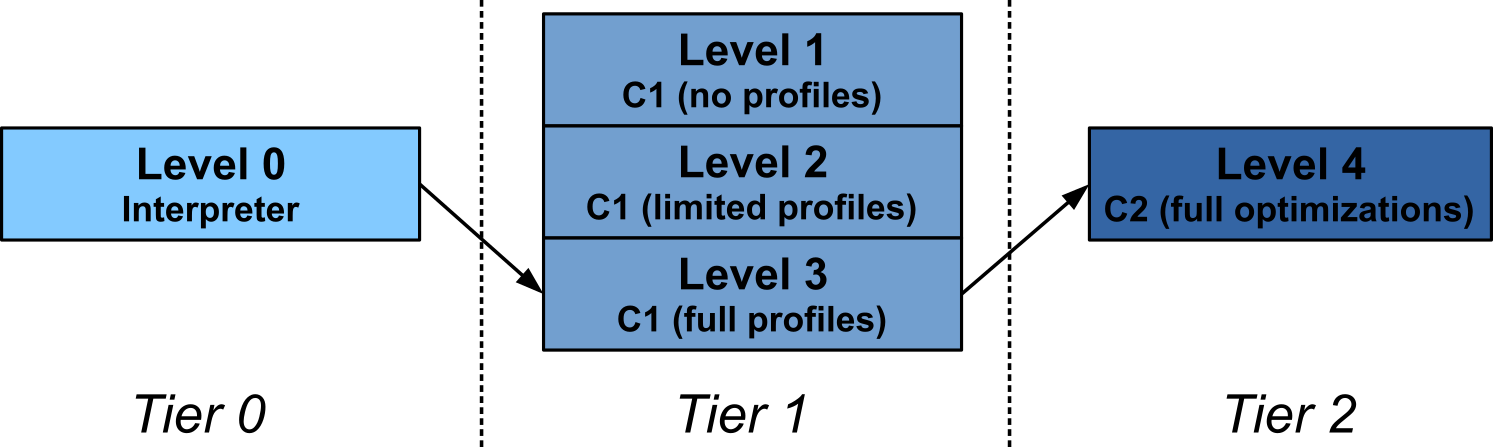
\includegraphics{figures/hs_tiers.png}
    \caption{Overview of compilation tiers}
    \label{f:hs_tiers}
  \end{center}
\end{figure}
\\
All methods start being executed at Tier 0, which denotes the interpreter.
The interpreter performs a template-based replacement, that is, for each bytecode instruction the interpreter emits a predefined assembly code snippet.
During execution, the assembly code is also profiled. The snippets also contain structures to gather method information like execution counters or loop back-branches. If a counter exceeds a predefined threshold, the method is considered \textit{hot} and a call back to the JVM is initiated that usually results in a compilation at a higher tier.
\\\\
The standard behavior of HotSpot is to proceed with Level 3 (Tier 3). The method gets compiled with C1, also referred to as \textit{client} compiler.
C1's goal is to provide a fast compilation with a low memory footprint.
The client compiler performs simple optimizations such as constant folding, null check elimination, and method inlining based on the information gathered during interpretation. 
Most of the classes and methods have already been used in the interpreter, allowing C1 to inline them to avoid costly invocations.
More importantly, information about the program flow and state are gathered. This information contain for example which branches get taken or the final types of dynamically typed objects. 
For example, if certain branches were not taken during execution, further compilations might abstain from compiling these branches and replace them with static code to provide a faster method execution time (see the example in Listing \ref{l:branchexample}). The uncommon branch includes an \textit{uncommon trap} which notifies the JVM that an assumption does not hold anymore. This then leads to so called \textit{deoptimizations} which are further explained in the separate Section \ref{s:deoptimizations}.
\begin{lstlisting}[float,caption=Example that shows potential compilation based on profiling information,label=l:branchexample,language=Java]
public static void m(int i) {
    if ( i == 0 ) { // very common branch (a)
        Math.sin(0);
    } else { // very uncommon branch (b)
        Math.sin(pi + i)
    }
}
// ---------------------------------------------
// If the JVM realizes based on profiling information,
// that branch (a) is taken all the time:
// compiler could compile the method as follows:
// ---------------------------------------------
public static void m(int i) {
    if ( i != 0 ) // very common branch (a)
        // UNCOMMON TRAP, call to JVM
    return 0; // result of sin(0)
}
\end{lstlisting}
\\\\
Level 1 and Level 2 include the same optimizations but offer no or less profiling information and are used in special cases. Code compiled at these levels is significantly faster than Level 3 because it needs to execute none or little instructions creating and managing the profiles. Since the profiles generated by C1 are further used in C2, HotSpot is usually interested in creating full profiles and therefore uses Level 3.
There are, however, rare instances where a compilation of Level 1 or Level 2 is triggered. For example, if enough profiles are available and a method can not be compiled by a higher tier, HotSpot might recompile the method with Tier 2 to get faster code until the higher tier compiler is available again. A compiler can become unavailable if its compilation queue exceeds a certain threshold. Also, if a method is simple, it may be compiled at Level 1.
\\\\
More information about C1 can be found in \cite{client_compiler_talk} and \cite{client_compiler}.
\\\\
Eventually, when further compile thresholds are exceeded, the JVM compiles the method with C2, also known as the \textit{server} compiler.
The server compiler uses the profiles gathered in Tier 0 and Tier 3 and produces highly optimized code. C2 includes far more and more complex optimizations like loop unrolling, common subexpression elimination and elimination of range and null checks. It performs optimistic method inlining, for example by converting some virtual calls to static calls. It relies heavily on the profiling information and richer profiles allow the compiler to do more and better optimizations.
While the code quality of C2 is a lot better than C1 this comes at the cost of compile time. A more detailed look at the server compiler can be found in \cite{server_compiler}.
Figure \ref{f:hs_tiers} gives a short overview as well as showing the standard transitions.
\\\\
The naming scheme \textit{client/server} is due to historical reasons when tiered compilation was not available and users had to choose the JIT compiler via a HotSpot command line flag. The \textit{client} compiler was meant to be used for interactive client programs with graphical user interfaces where response time is more important than peak performance. For long running server applications, the highly optimized but slower \textit{server} compiler was the choice suggested. 
\\\\
Tiered compilation was introduced to improve start-up performance of the JVM.
Starting with the interpreter results in instantaneous execution (i.e. a method is executed right away as there is no delay caused by the method's compilation). Also, there are always methods that are executed infrequently. For these, the compilation overhead can exceed the performance gain that results from having a compiled version of the method. C1 allows the JVM to have optimized code available early on. That code can be used to create a richer profile which is then used by the C2 compiler later on. Ideally this profile already contains most of the program flow and the assumptions made by C2 hold. If that is not the case, the JVM might need to go back, gather more profiles and compile the method again. In this case, being able to do quick compilations with C1 decreases the amount of C2 recompilations which are even more costly.

\section{Deoptimizations}
\label{s:deoptimizations}
Ideally a method is compiled by making use of as much profiling information as possible.
For example, since the profiling information is usually gathered in Levels 0 and 3, it can happen that a method compiled by C2 wants to execute a branch it never used before (again see Figure \ref{l:branchexample}).
In this case the information about this branch is not available in the profile and therefore have not been compiled into the C2-compiled code.
This is done to allow further even more optimistic optimization and to keep the compiled code smaller. So instead, the compiler places an uncommon trap at unused branches or unloaded classes which will get triggered in case they actually get used at a later time during execution.
\\\\
The JVM then stops execution of that method and returns control back to the interpreter. This process is called \textit{deoptimization} and considered very expensive. The previous interpreter state has to be restored and the method will be executed using the slow interpreter. Eventually the method might be recompiled with the newly gained information.

\section{On-Stack replacement}
\label{s:onstackreplacement}
In case a method contains a long running loop, counting the method invocations is not enough to determine the hotness of the method. The program still spends a significant amount of time in that method but because the invocation counter does not increase, no compilation is scheduled.
Therefore, HotSpot also counts loop back branches and when a threshold (see also Section \ref{s:compilethresholds}) is reached a compilation is invoked. The JVM then replaces the method's code directly on the program stack. HotSpot sets up a new stack frame for the compiled method which replaces the interpreters stack frame and execution will continue using the native method.
\\\\
This process is called \textit{on-stack replacement} and usually shortened to OSR. The Figure \ref{f:osr} presented in a talk by T. Rodriguez and K. Russel \cite{client_compiler_talk} gives a graphical representation.
The benefits of OSR will become more obvious when looking at the first example in Chapter \ref{c:motivation}.
\begin{figure}[ht]
  \begin{center}
    \centering
    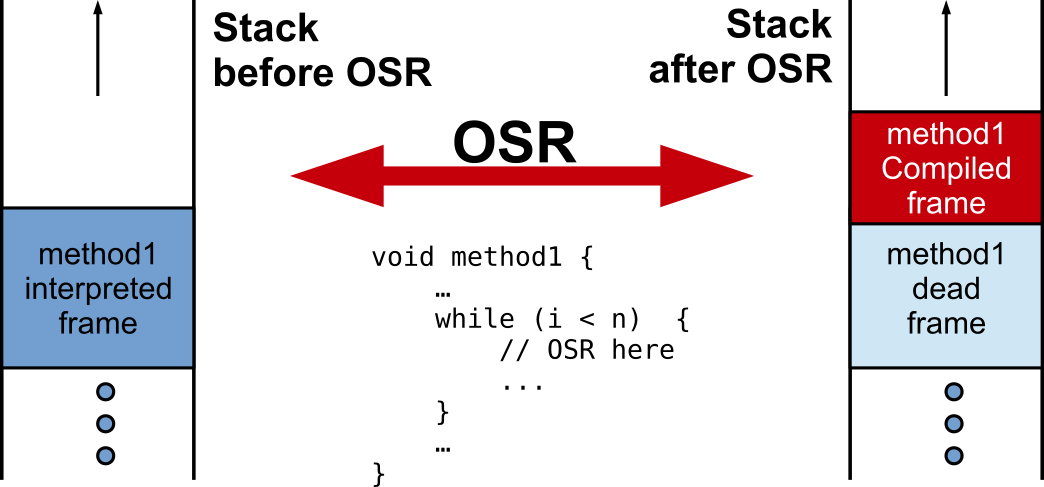
\includegraphics[width=0.6\textwidth]{figures/osr.png}
    \caption{Graphical schema of OSR}
    \label{f:osr}
  \end{center}
\end{figure}
\section{Compile thresholds}
\label{s:compilethresholds}
The transitions between the compilation levels (see Figure \ref{f:hs_tiers}) are chosen based on predefined constants called \textit{compile thresholds}. When running an instance of the JVM, one can specify them manually or use the ones provided. A list of thresholds and their default values relevant to this thesis are given in Appendix \ref{a:compilethresholds}.
The standard transitions from Level 0 to Level 3 and Level 3 to Level 4 happen when the following predicate returns true:
\begin{align*}
& i > TierXInvocationThreshold \ * \ s \\
 || \ (&i > TierXMinInvocationThreshold \ * \ s \ \&\& \ i \ + \ b \ > \ TierXCompileThreshold \ * \ s) 
\end{align*}
where $X$ is the next compile level (3 or 4), $i$ the number of method invocations, $b$ the number of backedges and $s$ a scaling coefficient (default = 1).
The thresholds are relative and individual for interpreter and compiler.
\\\\
On-stack replacement uses a simpler predicate:
$$b > TierXBackEdgeThreshold * s$$
\\\\
Note that there are further conditions influencing the compilation like the load on the compiler which will not be discussed.
